\section{GAMINR}
\label{sGAMINR}

\hypertarget{sGAMINRhy}{The}
GAMINR\index{GAMINR|textbf} module of NJOY is designed to
produce complete and accurate multigroup photoatomic
\index{photoatomic} (but not photonuclear) cross sections
from ENDF/B-IV and later data\cite{HUGO}, including
the newer formats developed for ENDF/B-VII.  Total, coherent,
incoherent, pair-production, and photoelectric cross sections can be
averaged using a variety of group structures\index{group structures}
and weighting functions.\index{weight functions}  The Legendre
components of the group-to-group coherent and incoherent scattering
cross sections are calculated using the form factors\cite{Hubbell}
\index{atomic form factors} now available in ENDF/B.  These form
factors account for the binding of the electron in its atom.
Consequently, the cross sections are accurate for energies as
low as 1 keV.  GAMINR also computes partial heating cross sections
or kinetic energy release in materials (KERMA\index{KERMA}) factors
for each reaction and sums them to obtain the total heating factor.
The resulting multigroup constants are written on an intermediate
interface file for later conversion to any desired format.
Photonuclear reactions\index{photonuclear reactions} such as
($\gamma$,n) are not computed by this module.

GAMINR differs from the previously used GAMLEG code\cite{GAMLEG} in
the following ways:\index{GAMLEG}
\begin{itemize}
\begin{singlespace}
\item Coherent form factors are processed thereby allowing higher
      Legendre components of the coherent scattering cross section to
      be produced.  GAMLEG processed the P$_0$ cross section only.

\item Incoherent structure factors are processed giving
      accurate results at low energies where the Klein-Nishina formula
      fails.

\item Heat-production cross sections (KERMA factors) are
      generated.

\item Variable dimensioning and dynamic storage allocation
      allow arbitrarily complex problems to be run.

\item GAMINR is much slower than GAMLEG since charge scaling
      of the incoherent matrix can no longer be used at all energies.
\end{singlespace}
\end{itemize}

This chapter describes the GAMINR module in NJOY2016.0.

\subsection{Description of ENDF/B Photon Interaction Files}
\label{ssGAMINR_Desc}

In the ENDF/B-IV and later photon interaction files, the
\index{photoatomic!coherent}
coherent scattering of photons by electrons is represented by
  \begin{equation}
    \sigma_C(E,E',\mu)\,dE'd\mu={{3\sigma_T} \over 8}(1+\mu^2)
    \,|F(q,Z)|^2\delta(E-E')\,dE'd\mu   \,\,,
  \label{eq1}
  \end{equation}

\noindent
where $E$ is the energy of the incident photon, $E'$ is the energy of
the scattered photon, $\mu$ is the scattering cosine, $\sigma_T$ is
the classical Thomson cross section (0.66524486 b),
\index{Thomson cross section}
$Z$ is the atomic number of the scattering atom, and $F$ is
the atomic form factor.  The coherent form factor is a function
of momentum transfer $q$ given by

  \begin{equation}
    q=2k\sqrt{{1-\mu} \over 2}   \,\,,
  \label{eq2}
  \end{equation}

\noindent
where $k$ is the energy in free-electron units ($k=E/511003.4$ eV), but $F$
is actually tabulated versus the quantity $x=20.60744q$.  The coherent
form factor is given as MT=502 in File 27.

Incoherent scattering\index{photoatomic!incoherent}
is represented by the expression

  \begin{equation}
    \sigma_I(E,E',\mu)\,dE'd\mu=S(q,Z)\,\sigma_{KN}(E,E',\mu)\,dE'd\mu \,\,,
  \label{eq3}
  \end{equation}
\vspace{0.5 pt}

\noindent
where $S$ is the incoherent scattering function and $\sigma_{KN}$ is the
free-electron Klein-Nishina cross section\index{Klein-Nishina}

  \begin{equation}
    \sigma_{KN}(E,E',\mu)={{3\sigma_T} \over {8k^2}}\biggl[{k \over k'} +
    {k' \over k} + 2\biggl({1 \over k}
    - {1 \over k'}\biggr) + \biggl( {1 \over k}
    - {1 \over k'} \biggr)^2 \biggr]   \,\,.
  \end{equation}
\vspace{0.5 pt}

\noindent
The scattering angle and momentum transfer for incoherent scattering
are given by

  \begin{equation}
    \mu=1+{1\over k}-{1 \over k'}  \,\,,
  \label{eq5}
  \end{equation}

\noindent
and

  \begin{equation}
    q=2k\sqrt{{1-\mu}\over 2} {{\sqrt{1+(k^2 +2k)(1-\mu)/2}}
    \over {1+k(1-\mu)}} \,\,.
  \label{eq6}
  \end{equation}
\vspace{0.5 pt}

\noindent
As was the case for coherent scattering, $S(q,Z)$ is actually tabulated
{\it vs.} $x=20.60744q$.  It is important to note that $S$ is essentially
equal to $Z$ for $x$ greater than $Z$.  The incoherent scattering function
is given as MT=504 in File 27.

The ENDF/B-IV and later photon interaction files also contain
tabulated cross sections for total, coherent, incoherent, pair
production, and photoelectric reactions.
\index{photoatomic!pair production}
\index{photoatomic!photoelectric}
They are given in File 23 as MT=501, 502, 504, 516, and 602
respectively (note however, starting with the ENDF/B-VI files, MT=602 data
appear in MT=522).  The coherent and incoherent cross sections were
obtained by the evaluator by integrating Eqs.~\ref{eq1} and
\ref{eq3} and are therefore redundant.  Due care must be taken
to avoid introducing inconsistencies.  Starting with ENDF/B-VI,
there are additional cross sections given for the partial
photoelectric reactions starting with MT=534.

%The existing photon interaction data libraries contain no
%photonuclear data.

\subsection{Calculational Method}
\label{ssGAMINR_CalcMethod}

The multigroup cross sections produced by GAMINR are defined as
follows:

  \begin{eqnarray}
    \sigma_{xg}&=&{{\int_g\sigma_x\,\phi_0(E)\,dE}
    \over {\int_g\phi_0(E)\,dE}} \,\,,\\
    \mbox{}\nonumber\\
    \sigma_{T\ell g}&=&{{\int_g\sigma_T(E)\,\phi_\ell(E)\,dE}
    \over {\int_g\phi_\ell(E)\,dE}} \,\,,\;\hbox{and}\\
    \mbox{}\nonumber\\
    \sigma_{x\ell g\rightarrow g'}&=&
    {{\int_g{\cal F}_{x\ell g'}(E)\,\sigma_x(E)\,\phi_\ell(E)\,dE}
    \over {\int_g\phi_\ell(E)\,dE}} \,\,.
  \end{eqnarray}

\noindent
In these expressions, $g$ represents an energy group for the initial
energy $E$, $g'$ is a group of final energies $E'$, $x$ stands for one
of the reaction types, $T$ denotes the total, and $\phi_\ell$ is a
Legendre component of a guess for the photon flux.  In the last equation,
${\cal F}$ is the ``feed function''; that is, the total normalized
probability of scattering from $E$ into group $g'$.  The feed function
for coherent scattering is

  \begin{eqnarray}
    {\cal F}_{C\ell g'}(E)
    &=&{{\int_{-1}^{+1}\sigma_C(E,E',\mu)\,P_\ell(\mu)\,d\mu}
    \over { \sigma_C(E)}}  \nonumber\\
    &=&{{\int_{-1}^{+1}(1-\mu^2)\,|F(x)|^2P_\ell(\mu)\,d\mu}\over
    {\int_{-1}^{+1}(1-\mu^2)\,|F(x)|^2d\mu}}  \,\,,
  \label{eq10}
  \end{eqnarray}

\noindent for $E$ in $g'$ and zero elsewhere.

Here $P_\ell (\mu)$ is a Legendre polynomial.  Note that
${\cal F}_{C0g'}=1$;  this
form assures that the coherent scattering cross sections are
consistent with the values tabulated in File 23.

For incoherent scattering,

  \begin{equation}
    {\cal F}_{I\ell g'}={{\int_{g'}S(q,Z)\,\sigma_{KN}(E,E',\mu)\,
    P_\ell(\mu)\,dE'} \over
    {\int_{g'}S(q,Z)\,\sigma_{KN}(E,E',\mu)\,dE'}}  \,\,.
  \label{eq11}
  \end{equation}

\noindent
Because $S$ is simply equal to $Z$ for high values of $q$, it is not
necessary to completely recompute the incoherent matrix when
processing a series of elements in the order of increasing $Z$.  GAMINR
automatically determines that some groups for element $Z_{now}$ can be
obtained from element $Z_{last}$ by scaling by $Z_{now}/Z_{last}$.

Finally, pair-production is represented as a $(\gamma,2\gamma)$
scattering event, where

  \begin{equation}
    {\cal F}_{PP\ell g'}(E)=\left\{
    \begin{array}{ll}
     2,&\mbox{if $g'$ includes 511003.4 eV;}\\
     0,&\mbox{otherwise\,\,.}
    \end{array}
    \right.
  \end{equation}

In addition, GAMINR computes multigroup heating cross sections or KERMA
\index{photoatomic!KERMA} factors as follows:

  \begin{equation}
    \sigma_{Hxg}={{\int_g\,[E-\overline{E}_x(E)]\,\sigma_x(E)\,\phi_0(E)\,dE}
    \over {\int_g\phi_o(E)\,dE}} \,\,,
  \end{equation}

\noindent
where $\overline{E}_x(E)$ is the average energy of photons scattered from
$E$ by reaction type $x$.  The average energies are computed using
  \begin{eqnarray}
    \overline{E}_C    &=& E\,\,,\\
    \overline{E}_{PP} &=& 1.022007*10^6 {\,\rm eV}\,\,,\\
    \overline{E}_{PE} &=& 0,\;\hbox{and}\\
    \overline{E}_I(E) &=& \int_0^\infty E'\,\sigma_I(E,E',\mu)\,dE
    '/\,\sigma_I(E)\,\,.
  \end{eqnarray}

These separate contributions to the heating cross section are summed
to get a quantity that can be combined with a calculated flux to
obtain the total heating rate.

\subsection{Integrals Involving Form Factors}
\label{ssGAMINR_FormFact}

The integrals of Eqs.~\ref{eq10} and \ref{eq11} that involve the form
factors are very difficult to perform because of the extreme forward peaking
of the scattering at high energies.  Fig.~\ref{fig1} illustrates the
problem for coherent scattering.

\begin{figure}[thb]\centering
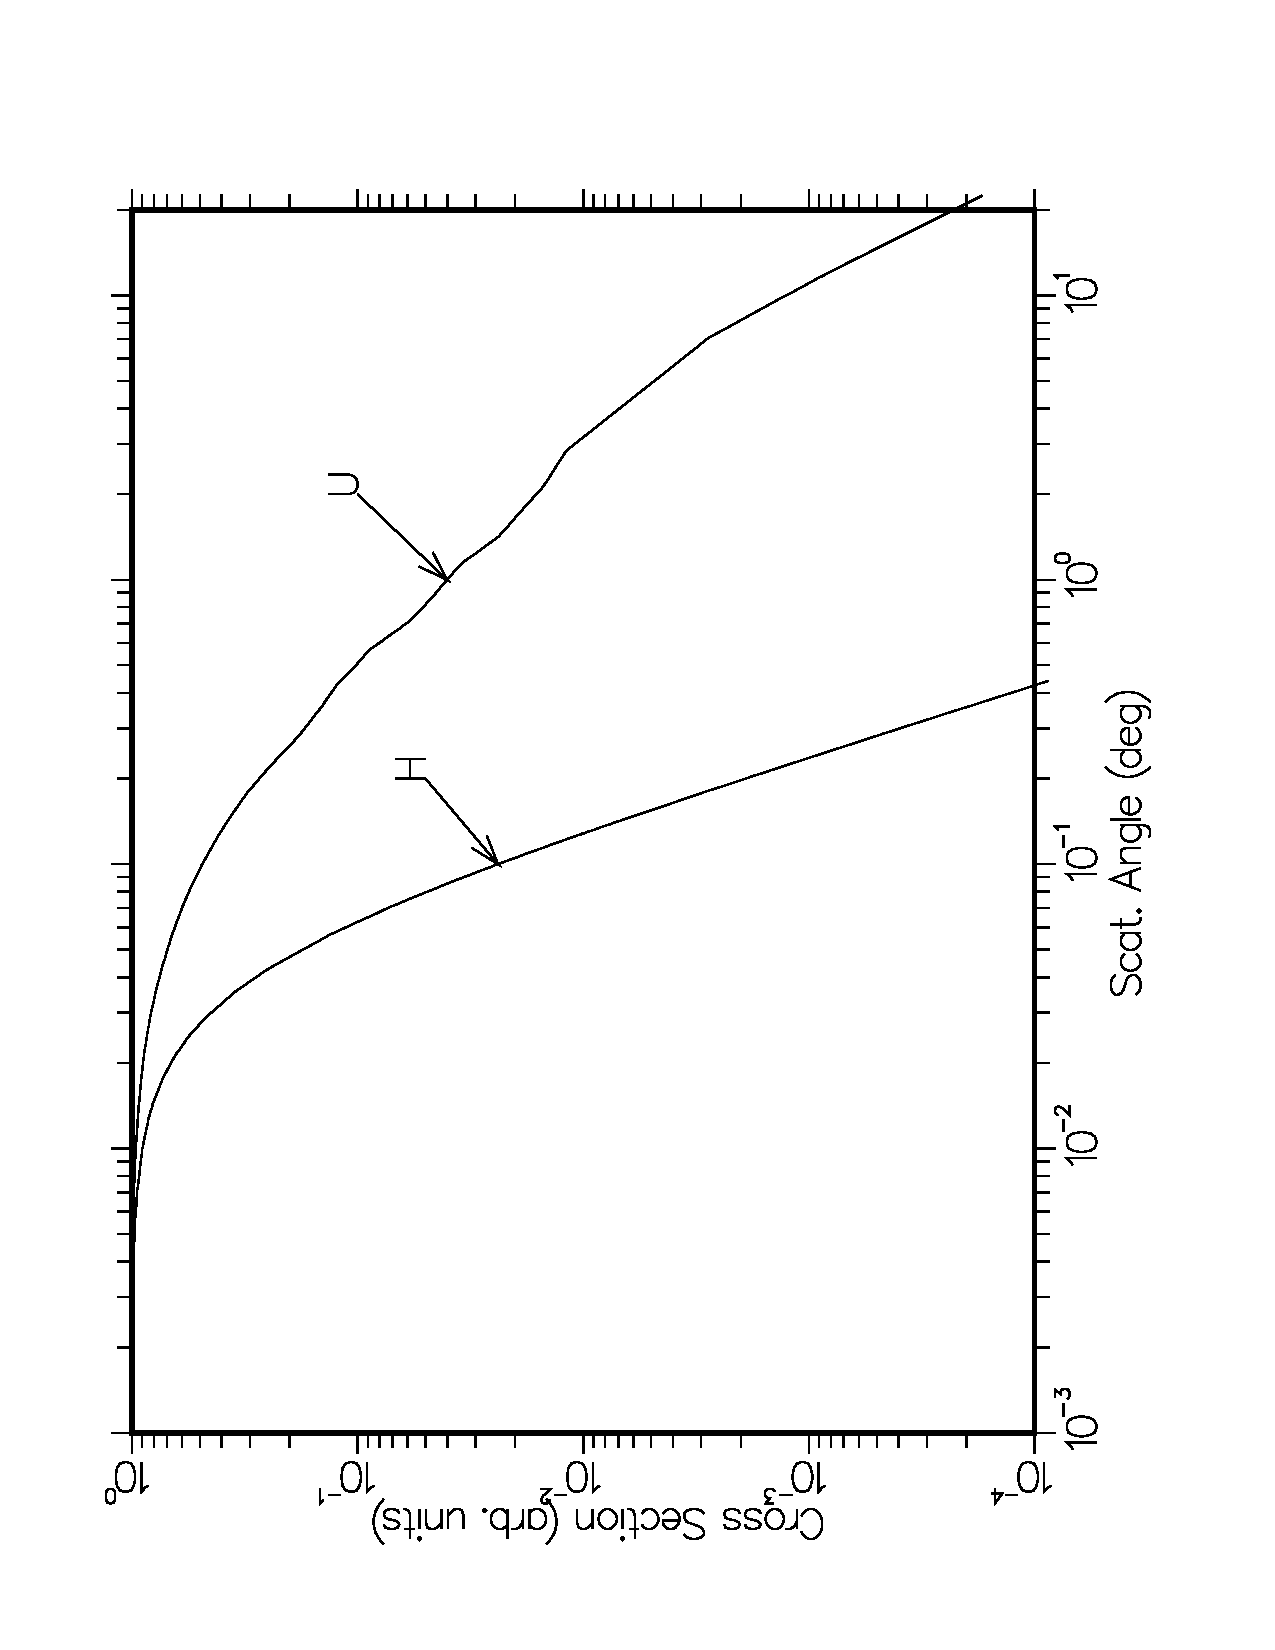
\includegraphics[keepaspectratio, height=3.5in, angle=270]{figs/gaminr1ack}
\caption[Photon coherent scattering angular distributions]{Angular distribution
 for coherent scattering from hydrogen and uranium at high photon energy.}
\label{fig1}
\end{figure}

For coherent scattering, the integral of Eq.~\ref{eq10} is broken up
into panels  by the tabulation values of $x$.  Each panel is integrated
in the $x$ domain using Lobatto quadrature of order 6 for $\ell=3$
or less and order 10 for larger Legendre orders.  Eq.~\ref{eq2}
is used to compute the $\mu$ value for each $x$ and to obtain the
Jacobian required.

Since $\mu$ is quadratic in $x$, the polynomial order of the integrand
in the numerator of Eq.~\ref{eq10} is $2\ell+2$ plus twice the polynomial
order of $F$ in the panel.  For $\ell=3$, the theory of Gaussian quadrature
implies that the integral will be exact if $F$ can be represented as a
quadratic function over the panel.

The incoherent integral of Eq.~\ref{eq11} is also broken up into panels,
but here the panels are defined by the union of the tabulation values
of $x$ and the momenta corresponding to the secondary-energy group
bounds.  The relationship between $x$, $\mu$, and secondary energy is given
in Eqs.~\ref{eq5} and \ref{eq6}.  This time, the integral is
performed {\it vs.} $E'$ using Lobatto quadrature\index{Lobatto quadrature}
of order 6 for $\ell$ less than or equal to 5 and order 10 for
larger $\ell$ values.

All form factors and structure factors are interpolated using
ENDF/B log-log interpolation as specified by the format.  However, the
cross sections in the file were evaluated using a special
log-log-quadratic scheme.  Ignoring this complication may lead to a 5\%
error in the incoherent cross section at 0.1 keV with a negligible
error at the higher energies that are of most practical
concern\cite{Hubbell}.

\subsection{Coding Details}
\label{ssGAMINR_details}

The main entry point is subroutine \cword{gaminr} exported by
module \cword{gaminm}\index{modules!gaminm@{\ty gaminm}}.
The code begins by reading the user's input.  It then locates the
position for the new material on the old GENDF\index{GENDF}
tape (if any) and copies the earlier results to the new output
tape.  The desired material is also located on the input
PENDF\index{PENDF} tape prepared previously using
\hyperlink{sRECONRhy}{RECONR}\index{RECONR}.
A new material header is then written onto the output tape leaving
the code ready to begin the loop over reaction types.

For each of the preset reaction types, GAMINR uses the panel logic
of \hyperlink{sGROUPRhy}{GROUPR}\index{GROUPR} to
average the cross sections (see the ``panel" discussion
in Section~\ref{ssGROUPR_GrpInt}).  If this is the first material
in a series of elements, the incoherent matrix is saved to a scratch area.
For subsequent materials, the higher energy matrix elements are obtained
by scaling these saved values by the appropriate $Z$ ratio.  The
resulting cross sections and group-to-group matrix elements are then
printed out and written to the output tape.  The heat production
contribution from each reaction is summed into a storage area.  After
all reactions have been processed for this material, a special pass
through the output logic is used to create a heating section using
MT=525 for ENDF/B-VI and later files or MT=525 for earlier
ENDF/B files.  Finally, the rest of the
old output tape is copied to the new output tape.  A description of the
format of the multigroup output tape will be found in the
\hyperlink{sGROUPRhy}{GROUPR} chapter
(see Section~\ref{ssGROUPR_GENDF}).

As with \cword{panel} in
\hyperlink{sGROUPRhy}{GROUPR}, \cword{gpanel}\index{gpanel@{\ty gpanel}}
integrates the triple product ${\cal F}{*}\sigma{*}\phi$.  The feed into
secondary group $g'$ for Legendre order $\ell$ from initial energy $E$
is computed in \cword{gtff}\index{gtff@{\ty gtff}} as described in
Section~\ref{ssGAMINR_FormFact} above.  Cross sections are read from
the PENDF tape (see
\cword{gtsig}\index{gtsig@{\ty gtsig}}).  Flux can be read in,
constant, or $1/E$ with high and low energy roll-offs (see
\cword{gnwtf}\index{gnwtf@{\ty gnwtf}} and
\cword{gtflx}\index{gtflx@{\ty gtflx}}).

\subsection{User Input}
\label{ssGAMINR_UserInp}

The following description of the user input is reproduced from
the comment cards at the beginning of the GAMINR module.
\index{GAMINR!GAMINR input}
\index{input!GAMINR}

\small
\begin{ccode}

   !---input specifications (free format)---------------------------
   !
   ! card1
   !    nendf   unit for endf tape
   !    npend   unit for pendf tape
   !    ngam1   unit for input ngam tape (default=0)
   !    ngam2   unit for output ngam tape (default=0)
   ! card2
   !    matb    material to be processed
   !            input materials in ascending order
   !    igg     gamma group structure option
   !    iwt     weight function option
   !    lord    legendre order
   !    iprint  print option (0/1=minimum/maximum) (default=1)
   ! card3
   !    title   run label up to 80 characters (delimited by ',
   !            ended with /)
   ! card4      (igg=1 only)
   !    ngg     number of groups
   !    egg     ngg+1 group bounds (ev)
   ! card5      (iwt=1 only)
   !    wght    read weight function as tab1 record,
   !            this may span multiple lines and ends with a /.
   ! card6
   !    mfd     file to be processed
   !    mtd     section to be processed
   !    mtname  description of section to be processed
   !            repeat for all reactions desired
   !            mfd=0/ terminates this material
   !            mfd=-1/ is a flag to process all sections present
   !            for this material  (termination is automatic)
   ! card7
   !    matd    next mat number to be processed
   !            terminate gaminr run with matd=0.
   !
   !---options for input variables----------------------------------
   !
   !        igg     meaning
   !        ---     -------
   !         0      none
   !         1      arbitrary structure (read in)
   !         2      csewg 94-group structure
   !         3      lanl 12-group structure
   !         4      steiner 21-group gamma-ray structure
   !         5      straker 22-group structure
   !         6      lanl 48-group structure
   !         7      lanl 24-group structure
   !         8      vitamin-c 36-group structure
   !         9      vitamin-e 38-group structure
   !         10      vitamin-j 42-group structure
   !
   !        iwt     meaning
   !        ---     -------
   !         1      read in smooth weight function
   !         2      constant
   !         3      1/e + rolloffs
   !
   !------------------------------------------------------------------

\end{ccode}
\normalsize

The weight options allowed by GAMINR are a user defined function, a constant
weight option and a $1/E$ option with high and low energy roll-offs. For more
information, see the weight options in the \hyperlink{sGROUPRhy}{GROUPR} module.

Note that both an ENDF/B tape and a PENDF tape from
\hyperlink{sRECONRhy}{RECONR} are required.
Older, pre-ENDF/B-VI, photon interaction tapes are available from the Radiation
Shielding Information Computational Center (RSICC) at ORNL
as DLC7E (for ENDF/B-IV) or DLC-99/HUGO (for ENDF/B-V).
A photoatomic library in ENDF-6 format based on DLC-99 is available
from the National Nuclear Data Center (NNDC) at the Brookhaven National
Laboratory.  The latest photoatomic library is also available
from the NNDC.  Material numbers (\cword{matb}) are simply the element
$Z$ number for versions IV and V;  they are equal to $100{*}Z$ for
ENDF-6 formatted files.  The values of \cword{matd} on card 7 should
be given in increasing order for maximum economy.  The normal mode
of operation uses \cword{mfd}$=-1$.  This automatically processes
MT=501, 502, 504, 516, 522, and 525.  For pre-ENDF-6 formatted files,
the photoelectric cross section is changed from 522 to 602, and the
heating cross section is changed from 525 to 621.

The following sample run prepares a GENDF tape for two elements.
The numbers on the left are for reference; they are not part of the input.

\small
\begin{ccode}

  1.   reconr
  2.   20 21/
  3.   'pendf tape for 2 elements from ENDF/B-VII'/
  4.   100 1 0/
  5.   .001 0./
  6.   '1-hydrogen'/
  7.   9200 1 0/
  8.   .001 0./
  9.   '92-uranium'/
 10.   0/
 11.   gaminr
 12.   20 21 0 22/
 13.   100 7 3 4 0/
 14.   '24-group photon interaction library'/
 15.   -1/
 16.   9200/
 17.   -1/
 18.   0/
 19.   stop

\end{ccode}
\normalsize

On line 2, an ENDF/B tape containing File 23 has been
mounted on logical unit 20.  The title on line 3 will appear on the PENDF
tape.  Material 100 is hydrogen (lines 4-6) and material 9200 is uranium
(lines 7-9).  The element names on lines 8 and 11 will appear on the
PENDF tape in MF=1,MT=451.  Linearization is accurate to better
than 0.1\%.  A more complete description of
\hyperlink{sRECONRhy}{RECONR's} input may be found in
Section~\ref{ssRECONR_inp}.

GAMINR uses the same ENDF tape as \hyperlink{sRECONRhy}{RECONR}
(actually only MF=27 is read
by GAMINR), but GAMINR also reads the
\hyperlink{sRECONRhy}{RECONR} output tape on unit 21.
The GAMINR GENDF tape will be on unit 22.  Card 13 specifies hydrogen
as the first material, 24 groups, $1/E$ weight with roll-offs,
Legendre components through P$_3$, and the full printed output.  Cards 16
and 17 select the default list of reaction types.  Card 16 specifies
uranium as the second material to be processed, and line 18 terminates
the element loop and the GAMINR run.

Figs.~\ref{fig2} and \ref{fig3} illustrate plots of the results of this
sample run.  These graphs were made using the
\hyperlink{sDTFRhy}{DTFR} and \hyperlink{sVIEWRhy}{VIEWR} modules.

\begin{figure}[p]\centering
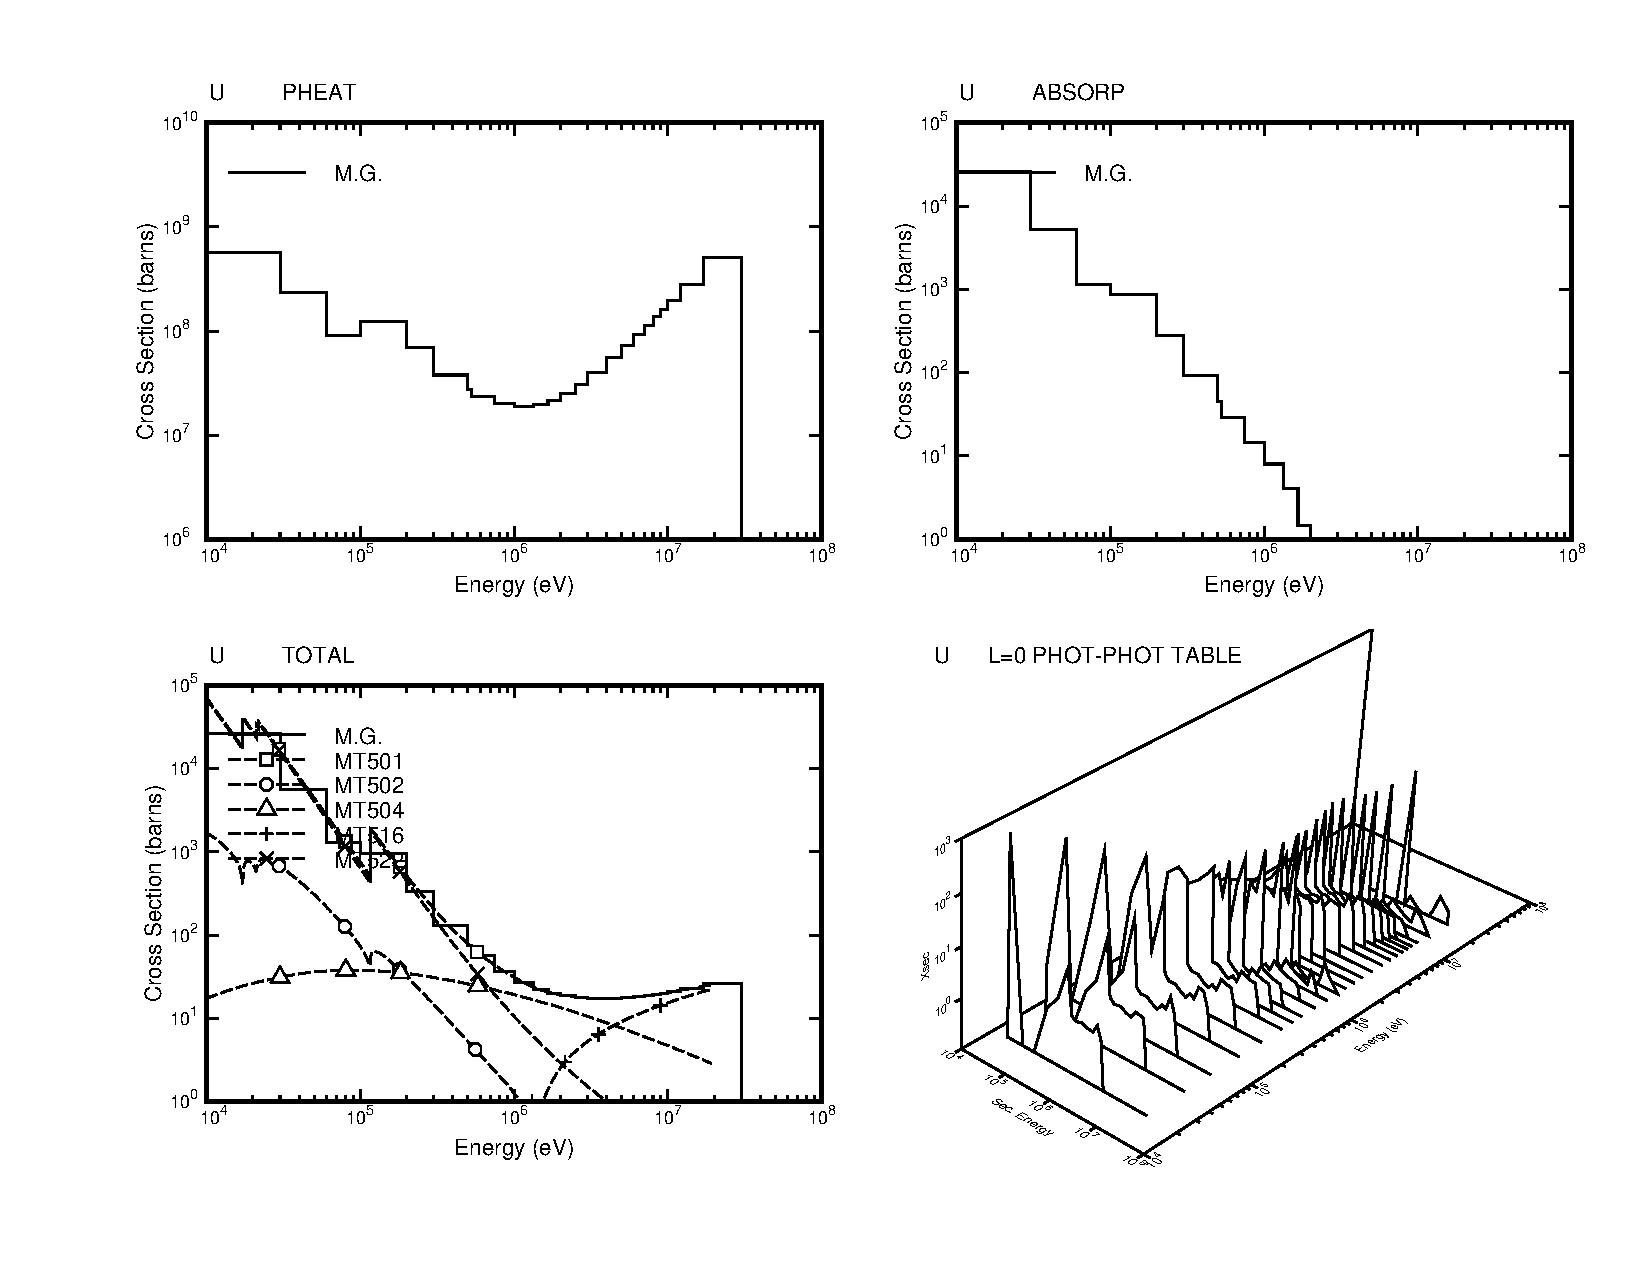
\includegraphics[keepaspectratio, width=4.5in, angle=0]{figs/gaminr2ack}
\caption[Photon interaction cross sections for uranium]{Plots of the photon
 interaction cross sections and the photon scattering distribution for uranium
 showing both 24-group and continuous cross sections.  Note the prominent
 photoelectric absorption edge near 100 keV.}
\label{fig2}
\end{figure}

\begin{figure}[p]\centering
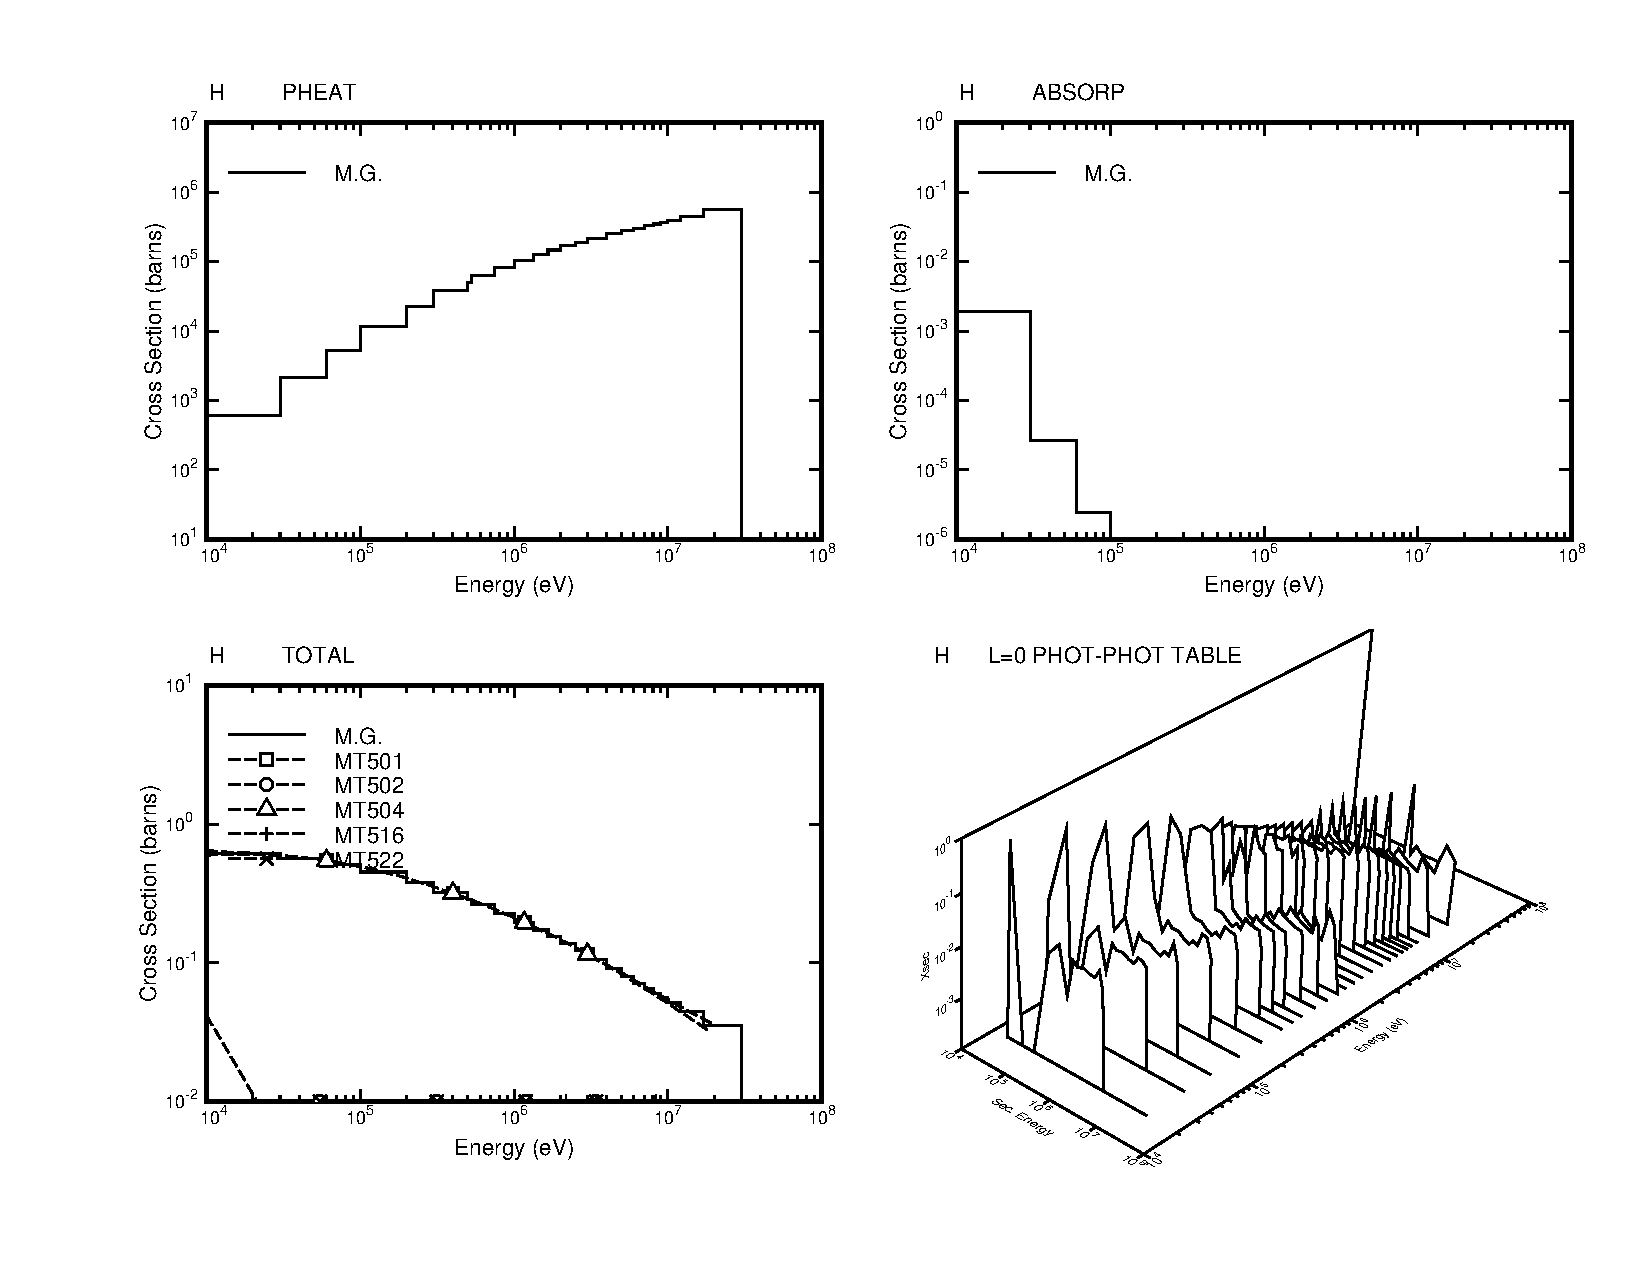
\includegraphics[keepaspectratio, width=4.5in, angle=0]{figs/gaminr3ack}
\caption[Photon interaction cross sections for hydrogen]{Plots of the photon
 interaction cross sections and the photon scattering distribution for hydrogen
 showing both 24-group and continuous cross sections.  The cross sections
 are simpler for this case.}
\label{fig3}
\end{figure}

Starting with ENDF/B-VI, the photon interaction (or photoatomic)
files contain detailed photoelectric cross sections, not just
the MT=522 total photoelectric cross section.  These photoelectric
cross sections have MT numbers starting with 534.  As an example,
Fig.~\ref{shells} shows the first 9 partial cross sections for
uranium --- the K, L, and M subshells --- taken from ENDF/B-VII.
GAMINR input is somewhat more complicated when these reactions
are included because they are different for every element.

\begin{figure}[thb]\centering
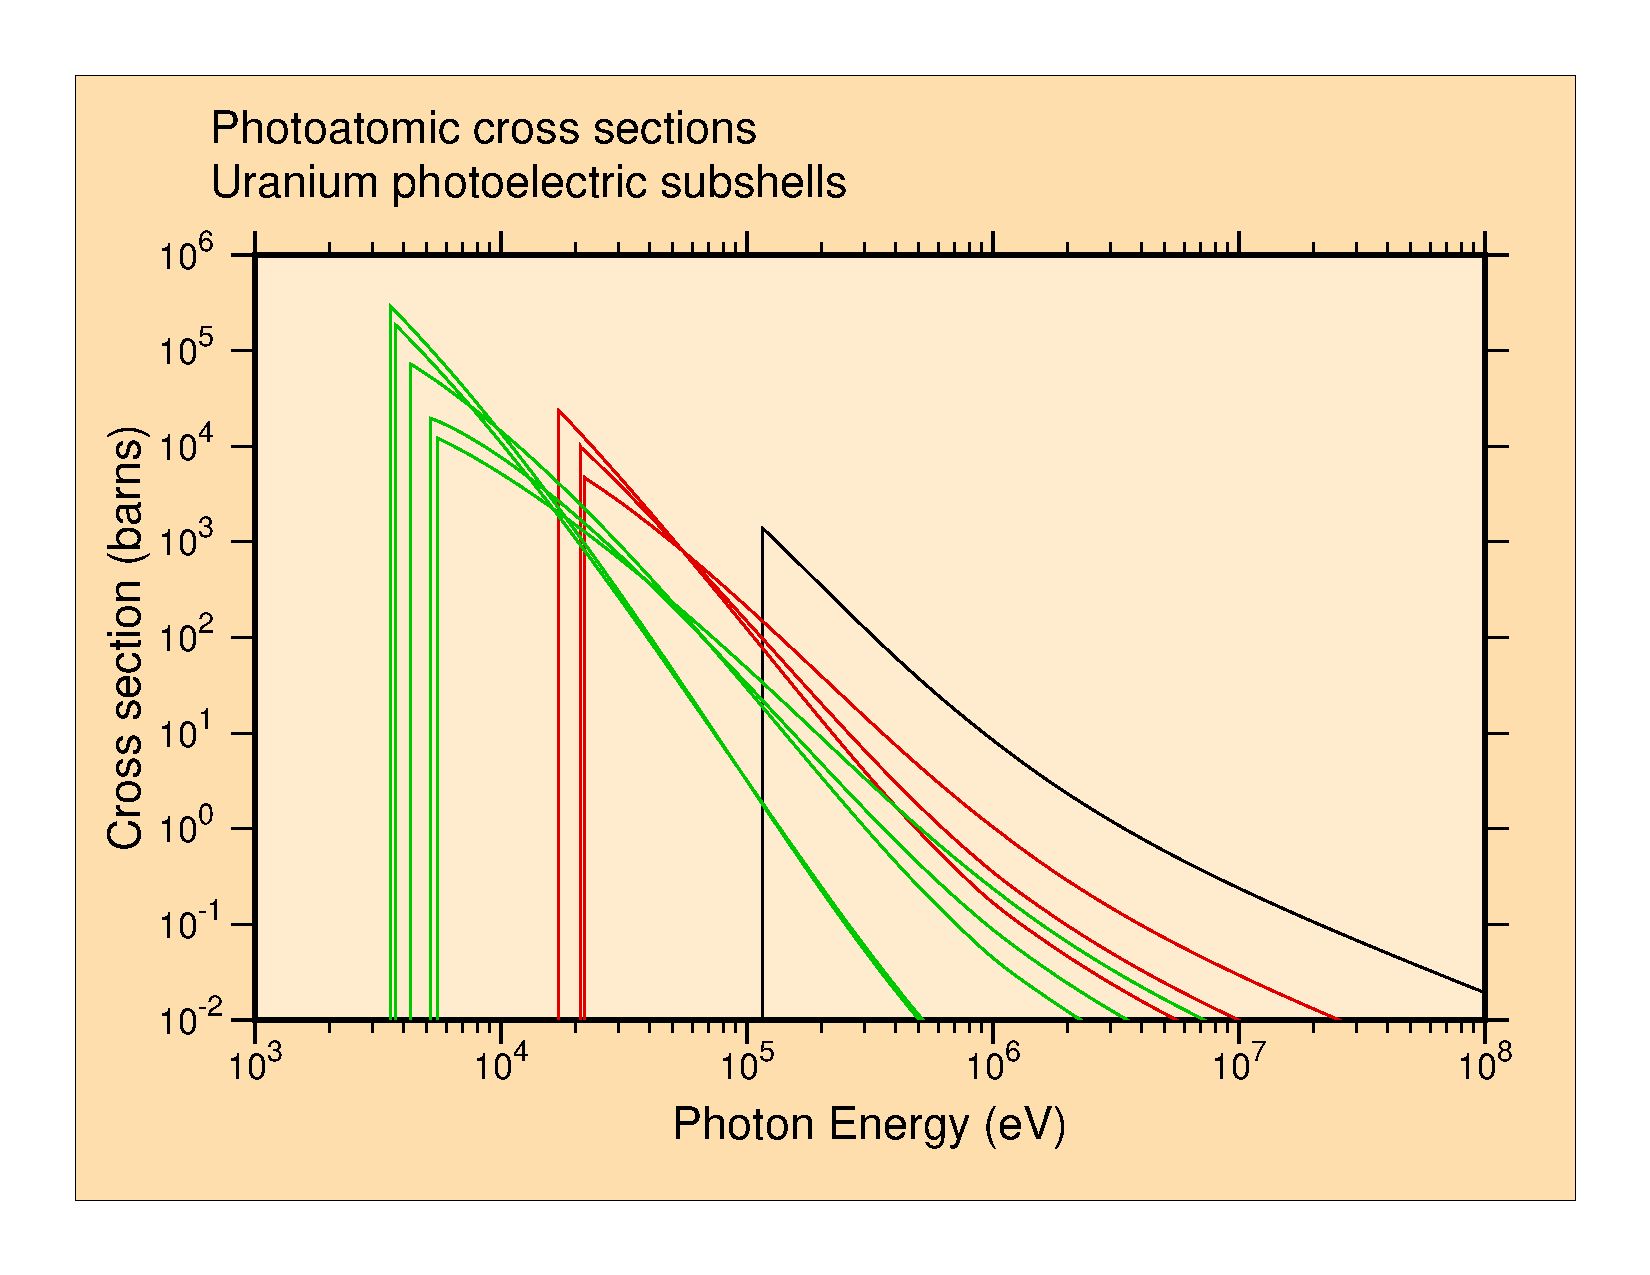
\includegraphics[keepaspectratio, width=4.0in,angle=0]{figs/gaminr4ack}
\caption[ENDF/B-VII.0 Uranium photoelectric subshell cross sections]{The
 first nine photoelectric subshell cross sections for uranium from
 ENDF/B-VII.0.  Black is the S subshell (1s$^{1/2}$), red is the L1, L2,
 and L3 subshells (2s$^{1/2}$, 2p$^{1/2}$, 2p$^{3/2}$), and green is the
 M1 through M5 subshells (3s$^{1/2}$, 3p$^{1/2}$, 3p$^{3/2}$, 3d$^{3/2}$,
 3d$^{5/2}$).}
\label{shells}
\end{figure}

\subsection{I/O Units}
\label{ssGAMINR_IO}

There are no scratch files used in GAMINR.  The only restriction
on the files assigned on line 1 of the user input is that \cword{ngam1} and
\cword{ngam2} must be in the same mode (that is, both binary or both
formatted).

\subsection{Error Messages}

\begin{description}
\begin{singlespace}

\item[\cword{error in genggp***illegal group structure}] ~\par
  Values of \cword{IGG} must lie between 1 and 10.

\item[\cword{error in genggp***too many groups.}] ~\par
  Increase the size of the global array \cword{egg} by changing the
  parameter \cword{ngmax}=400 located at the start of the module.

\item[\cword{error in gnwtf***illegal iwt}] ~\par
  Values of \cword{iwt} must lie between 1 and 3.

\item[\cword{error in gpanel***elo gt ehi.}] ~\par
  There is something wrong with the energy grids during integration
  over incident energy. This usually means there is a problem with
  the choice of \cword{rndoff} and/or \cword{delta}.  Be sure that
  \cword{rndoff}$<$1, \cword{delta}$>$1, and \cword{rndoff*delta}$<$1
  as represented on your machine.

\item[\cword{ERROR IN GTFF***ILLEGAL FILE TYPE.}] ~\par
  Only files 23 and 26 can be requested.

\item[\cword{error in gtff***illegal reaction for cross section=---}] ~\par
  Only reactions 501, 502, 504, 516, 602, and 621 (heat) can be requested
  for ENDF/B-IV or -V, or only 501, 502, 504, 516, 522, and 525 for
  ENDF/B-VI or VII.

\item[\cword{error in gtff***insufficient storage for form factor.}] ~\par
  This refers to the allocatable array \cword{pff} with size
  \cword{nwpff}=5000 defined in the main \cword{gaminr} routine.

\end{singlespace}
\end{description}

\cleardoublepage

